\documentclass[12pt, letterpaper]{article}
\usepackage[utf8]{inputenc}
\usepackage{graphicx}
\usepackage[spanish]{babel}

\graphicspath{{img/}}
\selectlanguage{spanish}

\title{\textbf{Informe escrito de Proyecto de Programación II: Intérprete para HULK} }
\author{Eveliz Espinaco Milián}
\date{Grupo C112}

\begin{document}
\thispagestyle{empty} 
\maketitle

\vspace{4cm}
\begin{center}
    Primer año de Lic. en Ciencia de la Computación \\ Facultad de Matemática y Computación \\ Universidad de La Habana \\ Curso 2023-2024
\end{center}

\begin{figure}[h]
    \centering
    
\includegraphics[scale= 0.53]{R.jpg}
\end{figure}

\newpage

\tableofcontents
\newpage

\section{Introducción}

HULK es un lenguaje de programación imperativo, funcional, estático y fuertemente tipado. Casi todas las instrucciones en HULK son expresiones. En el presente 
proyecto se implementará un intérprete de un subconjunto, de dicho lenguaje de programación,  compuesto solamente de expresiones que pueden escribirse en una 
única línea. Cada tipo de expresión del HULK es tratada en una clase, por lo que abordaremos toda su funcionalidad a la par que explicamos el funcionamiento del 
intérprete. Para ello nos apoyaremos de una gran variedad de ejemplos, desde los más sencillos hasta otros más complejos, y como es de suponer todos los ejemplos 
son compilables para el programa.
\newpage

\section{Algoritmo del intérprete.}
El algoritmo de este intérprete consiste en una vez insertada la instrucción del usuario fijarla, con ayuda de expresiones regulares, en una estructura: function, 
let-in, print, if-else, llamados de función o operaciones de tipos: string, números o booleanos. Una vez caracterizada la línea se procede a parsearla de forma más 
específica para determinar los tokens del tipo y su retorno. Este proceso es recursivo, dado que en una misma instrucción pueden haber varios tipos implementados
uno dentro de otro, por lo que la labor del intérprete se convierte en ir descomponiendo la instrucción en un ente de tipo string, número o booleano, la línea del 
usuario se define en la estructura que primero se detecte según una jerarquía conveniente que se utiliza para este proceso. Los errores, en su mayoría, se revelan de 
la siguiente forma: los léxicos se van detectando a medida que se parsea la instrucción para separarla por tokens, los semánticos a la vez que se trabaja en el retorno 
del tipo y los sintáticos cuando no hubo coincidencia con ninguna expresión regular se procesede a hacer un análisis para determinar a que modelo quiso referirse el 
usuario. \\

\textbf{Ejemplo:}
\begin{figure}[h]
    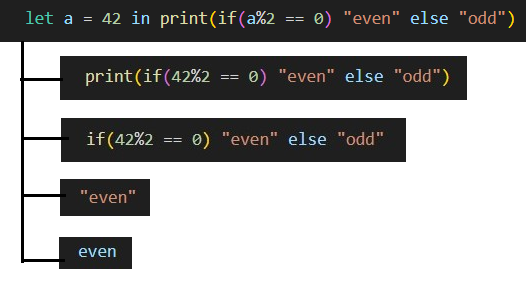
\includegraphics[scale= 0.90]{S.png}
\end{figure}

\newpage

\section{Clase HULK.}
Es la encargada de recibir la instrucción del usuario y establecer, a través de expresiones regulares, con que tipo tiene coincidencia su sintaxis, este  proceso lo 
realiza el método \textbf{Identificar} y según el resultado envía la instrucción a la clase encargada de trabajar esa estructura o al método \textbf{ErrorSintáctico} 
para darle una rectificación al usuario lo más detallada posible. Hasta que la expresión no coincida con una estructura string, números o booleano, o las combinaciones
de las operaciones en las que estos actúan (como es de suponer estos tipos están en el reglón más bajo de jerarquía definida para clasificar la línea introducida por el 
usuario) el método Identificar se seguirá llamando recursivo, pasándose en lugar de la instrucción original una nueva instrucción en la que la estructura detectada 
mutó a su retorno. \\ \\

\textbf{\underline{Métodos que la conforman: }} 

\begin{itemize}
    \item Identificar.  
    \item ErrorSintáctico.
\end{itemize}
\newpage

\section{Clase Utiles1 y Clase Utiles2}
Estas clases contiene métodos que se utilizan en el parseo de tipos, por tanto de ellas heredan otras clases. \\ 

\textbf{\underline{Métodos que conforman la clase Utiles1: }} 

\begin{itemize}

    \item Paréntesis que cierra: la utilizan varias clases como If-Else para determinar hasta donde llega la condición boolena del if. El método print para definir su cuerpo y otras estructuras que tienen en su sintaxis paréntesis.
    \item Ignorar: Este método recibe la posición de comillas dobles de un string y devuelve la posición de las comillas dobles que la cierran. Se utiliza en el parseo de varías estructuras, dado que un string puede tener palabras claves y otros identificadores y esto puede provocar errores sino son ignorados.

\end{itemize}

La clase Utiles2 es utilizada por las clases Let-in y Function, por lo que ambas clases heredan de Utiles2 y a la vez esta herda de Utiles1. \\ 

\textbf{\underline{Métodos que conforman la clase Utiles2:}} 

\begin{itemize}
    \item Es palabra reservada: comprueba si un string es una palabra reservada de HULK.
    \item Es nombre válido: comprueba que un string sea válido como identificador.
    \item Variables X Valor: Lo utiliza la clase Let-in para cambiar en el cuerpo de esta estructura el nombre de una variable por su valor, y también se utiliza con los llamados de funciones para cambiar en el cuerpo de una función el nombre de los parámetros por el valor introducido en la llamada.
\end{itemize}
\newpage

\section{Clase Expresión}
El programa dispone de una clase llama Expresión donde se encuentra establecida una expresión regular para cada tipo, y el método que hará 
uso de la expresión para evalar que se cumpla la sintaxis básica del tipo. Que un patrón reconozca válida la instrucción no esculpa la 
instrucción de errores. Por ejemplo: \\
La línea: \textbf{ if(2\<(3+5)-6 “correcto” else “incorrecto”} será reconocida por la expresión regular destinada para el tipo condicional 
if-else como válida, ya que la expresión regular está orientada a buscar que aparezcan todos los identificadores de la sintaxis del tipo, 
en este caso “if” “(“ “)” “else”, en ese orden y como se puede apreciar en el ejemplo dichos identificadores están presente, y aun así la 
instrucción es incorrecta, de ahí la nececidad de hacer un parseo una vez identificado el tipo.
\newpage

\section{Clase Function}
Se encarga se las declaraciones de funciones y los llamados de funciones.

\textbf{\underline{Campos de clase: }} 
\begin{itemize}
    \item nombre funciones. 
    \item parámetros.
    \item cuerpo función.
\end{itemize}

\textbf{\underline{Métodos que la conforman: }} 
\begin{itemize}
    \item Declarar función: se encarga de separar los tokens de la declaración de función: el nombre, los parámetros (se convierte, en un array) y el cuerpo de la función y los guardar en sus respectivos campos de clase.
    \item Llamada: se ocupa de parsear la instrucción en busca de llamados de funciones declaradas. En caso de encontrar una llamada, la envía al método Return llamada y luego sustituye en la instrucción original la llamda por su retorno. 
    \item Return llamada: sustituye en el cuerpo de la función guardado en el campo de clase el nombre de los parámetros por su valor e invoca al método Identificar pasando el cuerpo como una instrucción.
\end{itemize}

\textbf{Ejemplos de declaraciones de funciones:}\\
\begin{figure}[h]
    \centering
    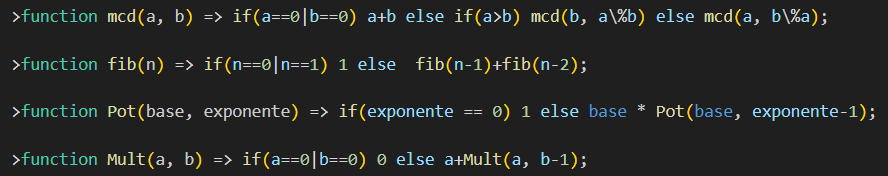
\includegraphics[scale= 0.90]{T.png}
\end{figure}     
\newpage

\section{Clase Let-in}
Esta estructura se utiliza para declarar variables y darles uso en la misma línea. Pueden declararse varias a la vez a través de la siguiente sintaxis: \\
(1) \textbf{let a = 3, b = 10 in a*b} \\
(2) \textbf{let a = 3 in (let b = 10 in a*b)} \\

Ambas estructuras son correctas. Pero el programa tomará como estructura principal la primera. La segunda no será más que una estructura let contenida dentro de otra, es decir en su cuerpo. Por tanto también son válidas la fusión de ambas sintaxis, como se muestra a continuación:  \\

\textbf{let a = 3, b = 10 in (let c = 6  in a*b*c)}  \\
\textbf{let a = 3, b = 10 in (let c = 6, d = 12 in a*b*c*d)} \\

\textbf{\underline{Métodos que la conforman: }} 
\begin{itemize}
    \item Return Let in: analiza la parte de la instrucción donde aparece una declaración de variable y sustituye dicha expresión por su retorno, para ello se auxilia del método Parse.
    \item Parse: Parsea la instrucción para separarla por tokens.
\end{itemize}
\newpage

\section{Clase Print}
Solo está formada por el método Return\_Print que se ocupa de sustituir toda la expresión print por el cuerpo de dicho tipo.
\newpage

\section{Clase If else}

\textbf{\underline{Métodos que la conforman: }} 
\begin{itemize}
    \item Return If else: Se auxilia del método Parse condition para obtener la condición del if, luego la envía al método Identificar para que desintegre otros tipos que puede tener la condición, como un llamado de función, una estructura print, entre otros y quede solo un true o false.
    \item Parse condition: parsea la instrucción y devuelve la condición.
    \item If condition is False: si la condición es falsa se devuelve el cuerpo del else, para ello solo habría que eliminar de la instrucción el substring que va desde if hasta la palabra else.  
    \item If condition is True: si la condición es true hay que hacer un parseo más complejo porque hay que definir con exactitud donde termina la estructura if-else.Se verifica si la estructura está dentro de paréntesis porque es una parte de una operación de tipos o si está dentro de un llamado de función o es simplemente la instrucción completa es una estructura if-else. En este punto del programa se descapta la existencia de tipos, let-in y print.
\end{itemize}
\newpage

\section{Clase Operar}
Esta clase es la encargada de las operaciones de los diferentes tipos(string, números, booleanos). \\

\textbf{\underline{Métodos que la conforman: }} 
\begin{itemize}
    \item Operaciones aritméticas: Para darle solución a las combinaciones de operaciones aritméticas se hace uso del Shunting Yard Algorthm. El cual consiste en convertir las expresiones matemáticas de notación infija, que es la forma que conocemos, a notación polaca inversa (RPN). Esta notación es una forma de escribir las expresión sin usar paréntesis ni prioridades de signos. \\
     Ejemplo: 3 * ( 2 + 5 ) en RPN se escribiría de la forma 3 2 5 + * \\
     Para su implementación se hace uso de dos listas, una simulando una pila.
    \item Operaciones con boleanos tipo1: Se ocupa de operar booleanes con true y false y los caracteres ! | y \&
    \item Operaciones con boleanos tipo2: opera los booleanos que están formados por las combinaciones de los caracteres ( ) | y \& e inecuaciones
    \item Operaciones con string: Concatena string.
\end{itemize}
\newpage

\section{Ejemplos}
\begin{figure}[h]
    \includegraphics[scale= 0.85]{X.png}
\end{figure}     
\newpage

\end{document}